
\chapter*{About this project}
\paragraph{Abstract:}
"Tech will transform from something we actively use to a more seamless integrated experience that is ‘on’ all the time." Daniel Baek, Co-founder of Nodes~\cite{nodes}. This paper proposes a new phone application that consists of the most important activities and features in demand for third level students around in Ireland. Feature's that can be accessed 24/7 and effortlessly by any user. The aim of this project was to create a suitable application that would benefit users in all aspects of their studies. Studies show that each household has an average of six devices connected to the internet. These consist of smart phones, laptops, computers and some household appliances. It was decided that this project would be developed for the most portable device held by users, mobile phones. Current deals with network vendors also allow the user to be connected to the internet through 3G or 4G technologies. All colleges maintain their own network for students also, this means that our application can be downloaded and used at all times.

\paragraph{Authors:}
This project was developed by two 4th year development students, Aaron Flanagan and Ciaran Brennan, as part of our Bachelors of Science honours degree in Applied Software Development.

\chapter*{Acknowledgements:}
We would like to acknowledge and thank Damien Costello for supervising this project. His expert advise and support helped guide this project to completion. We would also like to acknowledge the Department of Computer hnology for making this possible and helping us by providing support and any tools we needed during the development.

\chapter{Introduction}
The original idea for this project was the development of a facial recognition music application. The application would begin by capturing an image of the users face and running a mood capturing algorithm to determine the users mood, and it would then generate a play-list based on the users mood. This projects foreground was going to include an animated graphical user interface through the use of the JavaFX library made available by Oracle ~\cite{javafx}. The background was running a facial detection program that was described by the OpenCV Team~\cite{opencv}. This algorithm was going to build upon to include facial recognition as it only produced facial detection on screen by drawing shape around the users face, but this needed a feature extraction algorithm to complete it and that's when the idea hit a wall. After many weeks of research and study into the different approaches of facial recognition and feature extraction it was found that there was no Java binding libraries to OpenCV or resources that we could use. After a week of searching nothing was found that could help us, but because it was still early into the year the project idea had to be changed as to avoid further problems and time delay.

It was now October/November and the project was still at the beginning, GMIT hosted a hackathon for other colleges with software development courses to develop a project over a two day period. This time was used to explain the problem and come up with a new idea and build upon it until a clear project goal and list of possible features where decided on. Damien Costello was informed about the problem and advised the project idea could be changed while it was still possible, he was understanding and suggested a few ideas of projects to think about and do some research into. Out of those ideas came our student application idea, the development of an integrated mobile application solely for the purpose of third level students. He suggested doing something in augmented reality. It was thought upon and decided that the projects goal would be to build an application for students and include the augmented reality section as navigation around the college. A list was constructed of things that tend to be a problem for students and academic staff managing multiple years of students. Further research was done into the market to see what was already done and available. Many developers have developed applications with timetables or notes for your phone screen but we couldn't find any that contained all of these sections integrated into one application, or that where just institution specific. After decided what kind of application was to be built, the platform technology had to be chosen, this included research into the available systems. Finally a list of features had to be narrowed down to include in the project, what features would be more beneficial and would provide better context to the final application.

Further into this report will contain a breakdown and give an in-depth explanation to how the project was approached and developed, the different software and technologies used, an evaluation of the final product and notes taken by the developers about each feature and where they can be improved and why. The following sections will be discussed about the application:
\begin{itemize}
\item Methodology: This explains the production approach taken to developing the individual features of the application and how they where developed within the project time limit.
\item Technology review: This section discusses the various technologies used, both hardware and software. It explains how the project uses each component and gives an explanation to why this particular system/software was used and what is was used for.
\item System design: This section gives a breakdown of the projects architecture. How the system is built and how everything fits together.
\item System Evaluation: This section evaluates each feature of the application and compares the finished project to the original concept first described.
\item Conclusion: The final discussion about the project and evaluation of its finished state. Each section will be briefly concluded and it's main points will be stated.
\end{itemize}

This project can be found on Github under the name AaronFlanagan20 or CiaranB1992: https://github.com/AaronFlanagan20/CollegeEssentialsApp.
The repository contains a small ReadME file about how to download and run the application. The repository holds all the classes and native android files created and used by Android Studio to compile and run the project. Your computer or laptop must support virtualization, this can be checked by attempting to install Intel's hardware accelerator software or by checking for in the task manager of your machine. If said machine doesn't support it, you will be unable to run the emulator, instead you must plug in an android device with the developer options enabled.

\chapter{Methodology}
\section{Planning}
The first process of the project was planning everything that had to be done. This included when to hold meetings, what software to use for the development, what methodology to approach it with and how to test it appropriately. The first task finished was the creation of a project work flow to create a timely estimate of how long each feature will need and take into account other responsibilities the developers might have with other projects and reports. The project work flow or Gantt chart, was developed to show everything that needed to be done. It leaves out the section that assigns each individual developer to a particular area or feature because the list of features was not particularly large enough to scale out seven months of development and it was more beneficial to work as a pair due to the methodology taken. See Figure 1.

\section{Software Methodology}
Next was the decision of which methodology to pursue. It was decided this project would be developed based on Agile methodologies. "Agile methodology is an alternative to traditional project management, typically used in software development. It helps teams respond to unpredictability through incremental, iterative work cadences, known as sprints "~\cite{agile}. The traditional waterfall approach was not taken due to it's limitations put on each phase of the project. Each section had to completed in sequential order and time did not permit backtracking if a problem arised. Instead an incremental approach was taken. Both developers met up to discuss which feature to work on and to begin working on it by researching previously made work and reading through the Android documentation to find relative libraries available. This meant that each feature could be developed no matter how long it took to finish and different approaches could be taken. One feature may have taken a week at most to develop allowing  more time to improve it, while the next might have taken a month to complete. It also allowed more research and the ability to develop up-to date documentation and code during the development of each feature. If the code was re-factored or a different approach was taken that differed from the pre-determined plan specified at the beginning of this project, the developers where free to make the change and it was documented. During the development of that feature however, an iterative approach was taken. Each developer would plan, develop and test the feature and resort back to the original documentation to evaluate it. The same process would be taken again until the feature was eventually finished. At the end of each features cycle a meeting was held to discuss and evaluate it with the supervisor. These consisted of ideas on how to improve it or how to begin on the next. 

\section{Testing}
At the end of a features cycle, some testing was performed before moving on. This project used three forms of testing. The first form of testing is gradle, that is built into Android Studio. Gradle is a project build automation tool used to compile, test and run a native Java project and slow done build time and code freeze ups ~\cite{gradle}. It complies and runs the project within Android studio. Next used was CircleCI, CircleCI is a cloud platform used for continuous integration. Every time a commit was pushed up to the repository using git, CircleCI would pull down the code from Github and run a selection of tests on the new changes. If it passed the test the commit would integrate with the rest of the project on Github, if failed it would not be integrated until the problem was fixed via another commit to update or a revert to remove the new changes. Finally the developers wrote tests for the application using JUnit. JUnit is "A unit testing framework which is a central element of the Extreme Programming (XP) testing practice."~\cite{junit} JUnit was used to test the actions of components in the application to see if they performed the way they where suppose to, example if a pop-up box is meant to display on the press of a button. 
\begin{figure}
	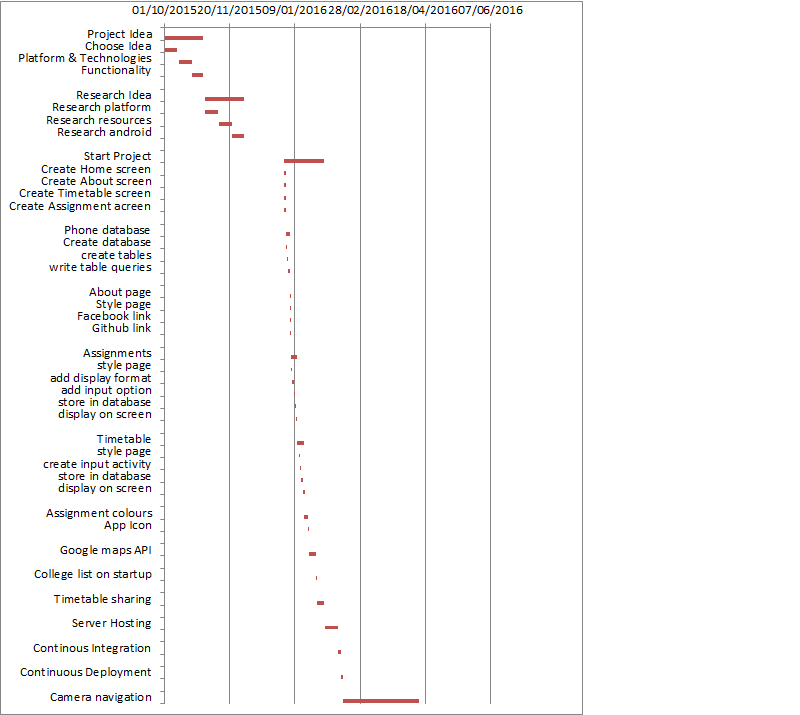
\includegraphics{img/gannt.png}
	\caption{Project Work Flow}
\end{figure}

\chapter{Technology Review}
About seven to ten pages.
\begin{itemize}
\item Describe each of the technologies you used at a conceptual level. Standards, Database Model (e.g. MongoDB, CouchDB), XMl, WSDL, JSON, JAXP.
\item Use references (IEEE format, e.g. [1]), Books, Papers, URLs (timestamp) – sources should be authoritative. 
\end{itemize}

\section{XML}
Here's some nicely formatted XML:
\begin{minted}{xml}
<this>
  <looks lookswhat="good">
    Good
  </looks>
</this>
\end{minted}

\chapter{System Design}
As many pages as needed.
\begin{itemize}
\item Architecture, UML etc. An overview of the different components of the system. Diagrams etc… Screen shots etc.
\end{itemize}

\begin{table}[h]
  \centering
  \begin{tabular}{x{2cm}p{3cm}}
    \toprule \\
    Column 1 & Column 2 \\
    \midrule \\
    Rows 2.1 & Row 2.2 \\
    \bottomrule
  \end{tabular}
  \caption{A table.}
  \label{table:mytable}
\end{table}

\chapter{System Evaluation}
As many pages as needed.
\begin{itemize}
\item Prove that your software is robust. How? Testing etc. 
\item Use performance benchmarks (space and time) if algorithmic.
\item Measure the outcomes / outputs of your system / software against the objectives from the Introduction.
\item Highlight any limitations or opportunities in your approach or technologies used.
\end{itemize}

\chapter{Conclusion}
About three pages.

\begin{itemize}
\item Briefly summarise your context and ob-jectives (a few lines).
\item Highlight your findings from the evalua-tion section / chapter and any opportuni-ties identified.
\end{itemize}

